\section{Methods}
In this paper, two different probabilistic formulations exist for the underlying edge importance model. All of these models rely upon the excellent \verb|Pyro| \cite{bingham_pyro_2018} framework for implementation and inference. Additionally, all GNN models are trained through the \verb|pytorch_geometric| \cite{fey_fast_2019} and \verb|pytorch| \cite{paszke_pytorch_2019} frameworks.

\subsection{Beta Model}
The first method used in this paper is a prior in which all Beta distributions are considered independent of each other. Specifically, we assume that $\mathcal{E}_i = E$ and that
\begin{align*}
	\mathcal{W}_i = \{\mathcal{W}_i(v_j , v_k) \mid (v,j, v_k) \in E\}
\end{align*}
with
\begin{align*}
	\mathcal{W}_i(v_j, v_k) = \mathbb{E}[Beta(\alpha_{j}, \beta_{k})]
\end{align*}
with $Beta(\alpha_{j,k}, \beta_{j, k})$ representing the prior Beta distribution on edge $(v_j, v_k)$ with specific parameters $\alpha_{j,k}$ and $\beta_{j,k}$. Note, we define the Beta distribution as
\begin{align*}
	\mathcal{P}(Beta(\alpha, \beta) = x) &= \frac{x^{\alpha - 1}(1-x)^{\beta - 1}}{\Beta(\alpha, \beta)} \\
	\Beta(\alpha, \beta) &= \frac{\Gamma(\alpha)\Gamma(\beta)}{\Gamma(\alpha + \beta)}
\end{align*}
where $\Gamma$ is the canonical Gamma function \cite{noauthor_continuous_nodate}. Given this, the goal of the interpretation task is to learn a variational family $q_{\phi}(H)$ that most closely resembles the posterior distribution when the categorical distribution
\begin{align*}
	\phi(v_i, \mathcal{X}, E, \mathcal{W}_i)
\end{align*}
is conditioned on the full model
\begin{align*}
	\phi(v_i, \mathcal{X}, E, \mathcal{W})
\end{align*}
where $\mathcal{W}(e) = 1$ for all $e \in E$. For the sake of this experiment, the posterior distribution is also assumed to be a set of Beta distributions but fully conditional on each other. The goal, then is to learn posterior values $\hat{\alpha}_{j,k}$ and $\hat{\beta}_{j,k}$. Given these values, the final explanation is
\begin{align*}
	\mathcal{W}_i(v_j, v_k) = \mathbb{E}[Beta(\hat{\alpha}_{j}, \hat{\beta}_{k})]
\end{align*}
which has an easily derived closed form.

\subsubsection{Interpretation of the Beta Model}
\begin{figure}[t]
	\centering
	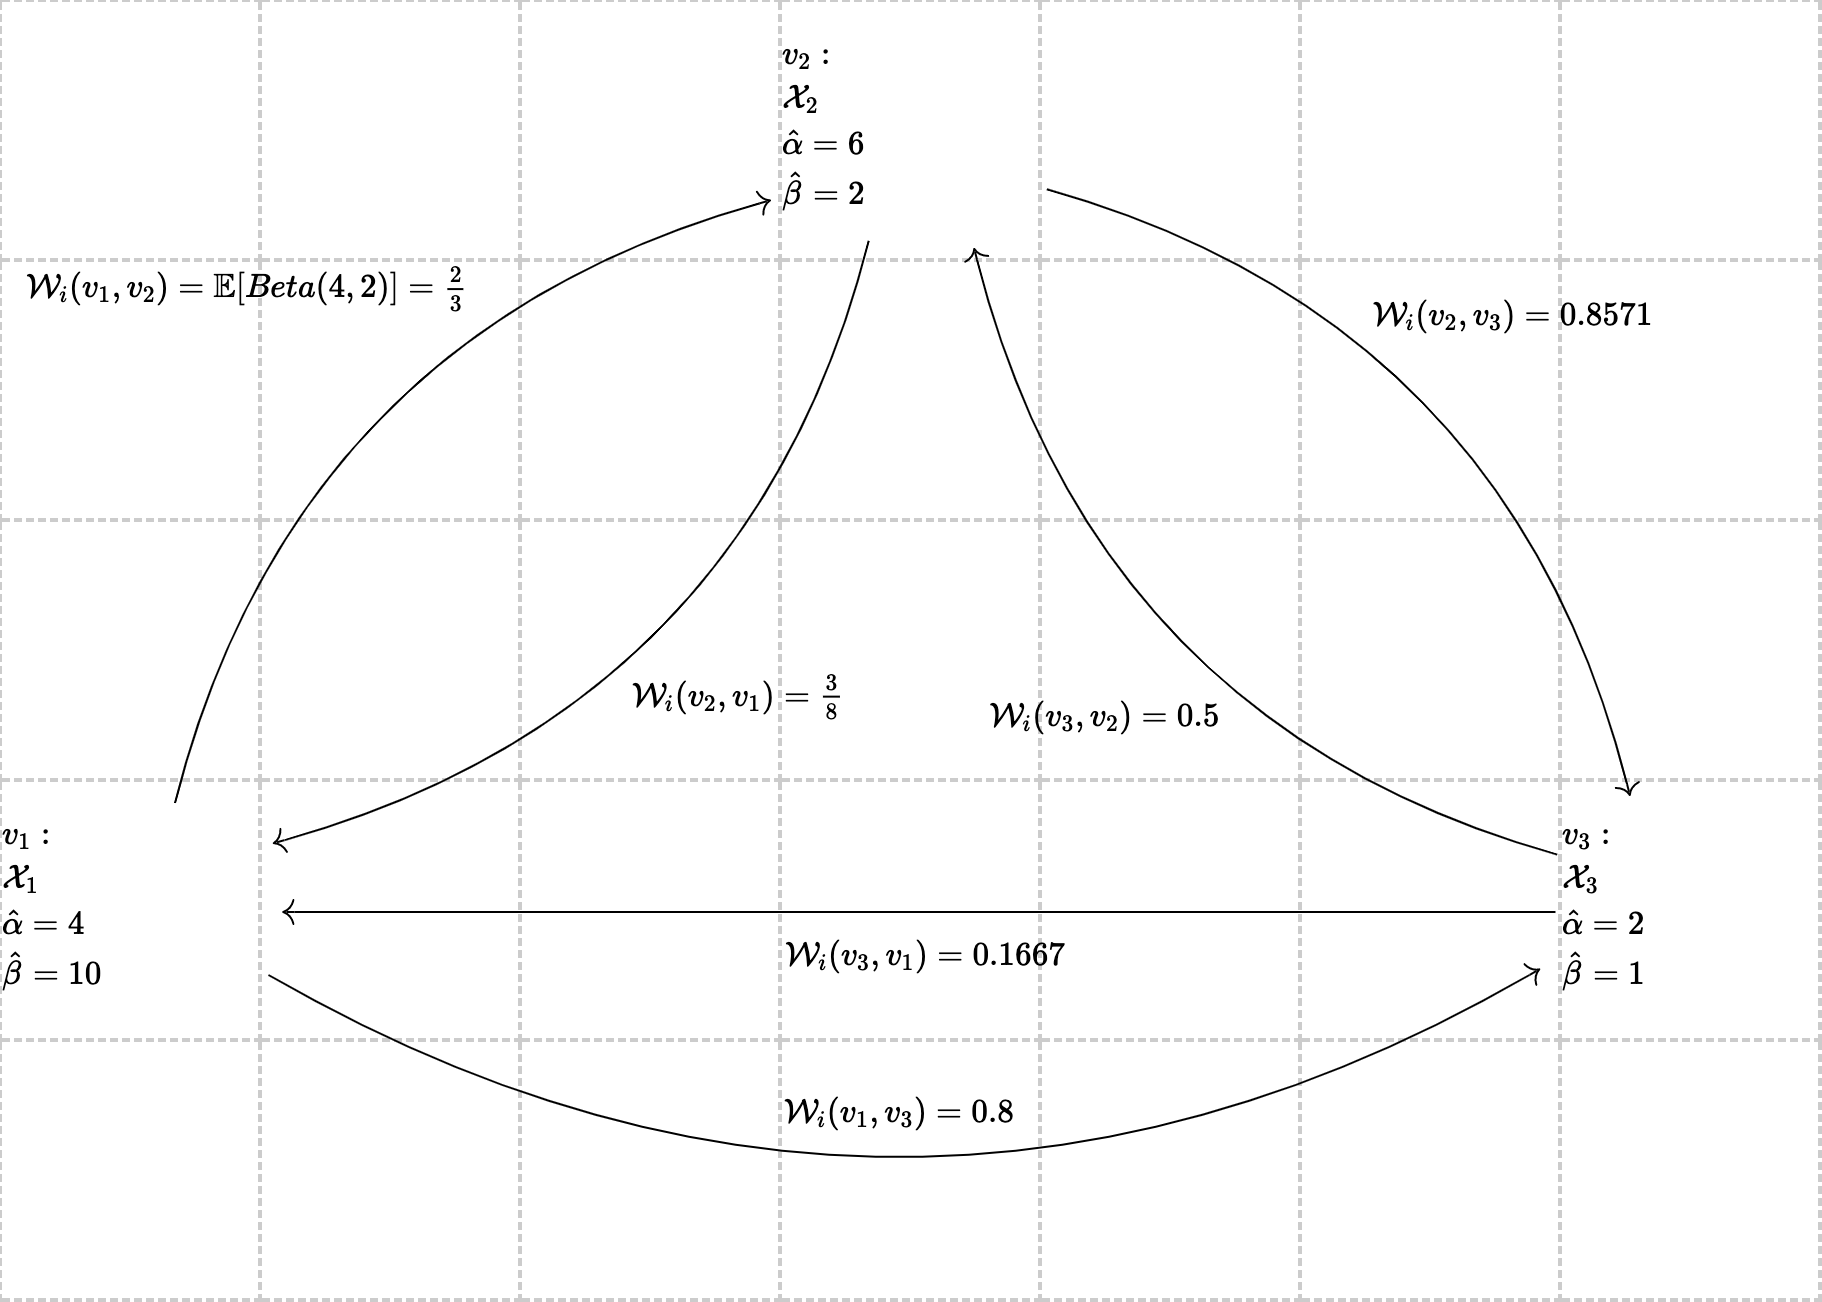
\includegraphics[width=\textwidth]{images/beta_ex.png}
	\caption{An example of a Beta posterior that shows information flowing from $v_1$ to $v_3$.}
	\label{fig:beta-ex}
\end{figure}
There is a wide array of literature on the use of Exponential-families for the modeling of edge weight priors. In particular, the work of Bolla \cite{bolla_estimating_2017} is important. In this work, edge weights are modeled by conditionally independent Beta distributions. The parameters of these Beta distributions are updated via a closed-form solution but it serves as a good model for prediction propagation of information or material from one node to another and converging on a steady-state for the propagation. In the case of GNNs, one can imagine the \verb|MSG| operation as the sending of information. The dense layers in the \verb|Upd| step, then, learn the weight to assign to each incoming and outgoing message. In this vein, the Beta model can approximate this "attention" that is paid in the \verb|Upd| step. Hence, the goal of this model is to serve as an approximation of this process and encode the steady-state flow of information in the model.
\begin{figure}[t]
	\centering
	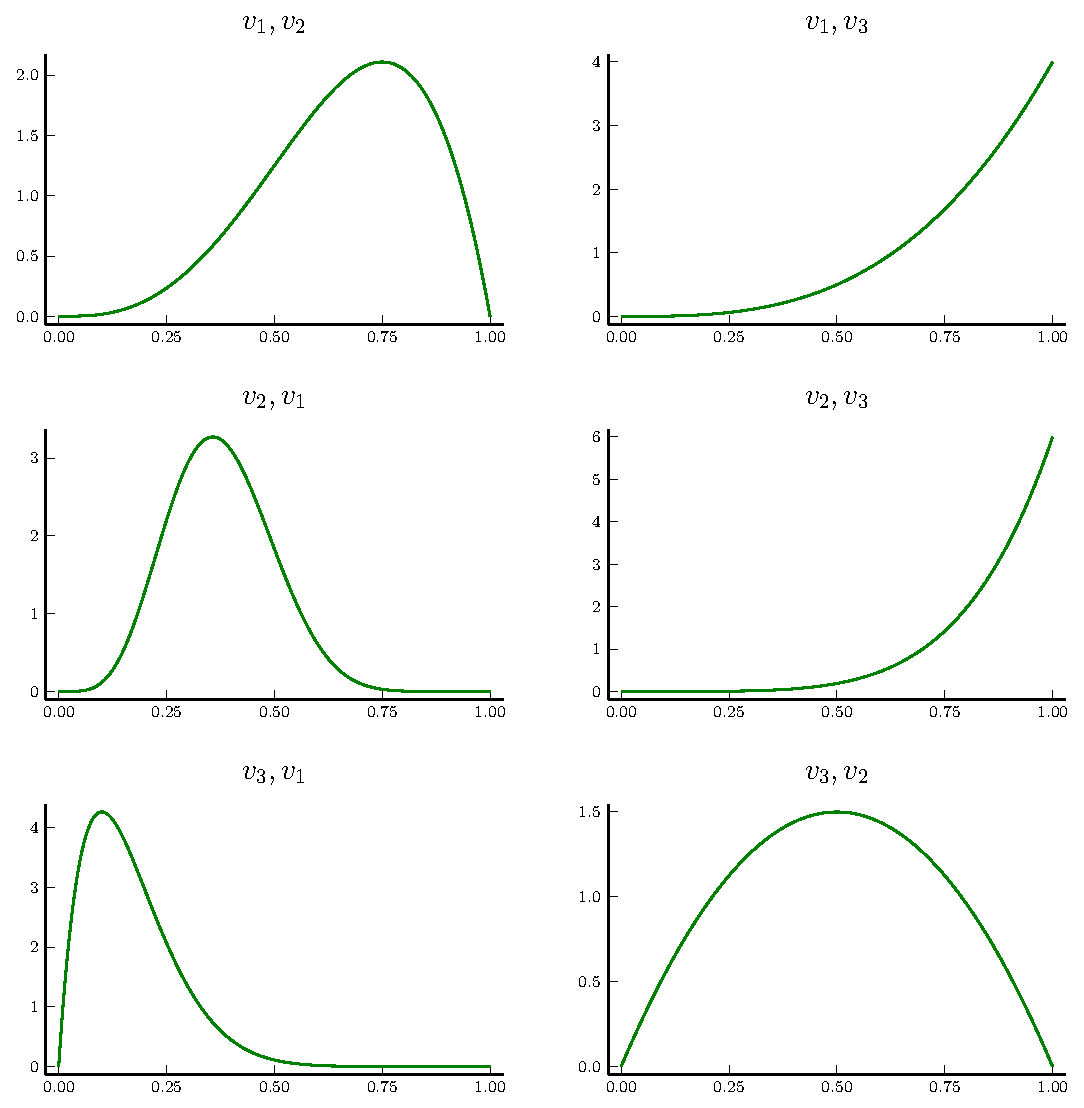
\includegraphics[width=0.8\textwidth]{images/beta_post.pdf}
	\caption{Posterior distributions for each edge in \ref{fig:beta-ex}}
	\label{fig:beta-ex-post}
\end{figure}

In this model, the $\alpha$ values serve to describe the affinity for information to flow out of a node while the $\beta$ values tend to describe the affinity for information to flow into the node. Together, they describe the steady state flow of information and perfectly describe many networks in which pathways of information lead to end-goal expression. Indeed, since GNNs tend to embed this type of information flow in a deep-learning setting, it serves to reason that such a prior would be a good encapsulation of the process of information flow, especially at steady state. A typical example of this is gene expression in biology \cite{petralia_new_2016} where paths of edges represent regulatory pathways directly. 

An example of this flow can be seen in figure \ref{fig:beta-ex}. In this figure, we consider a hypothetical posterior for this model and demonstrate how it describes the flow of information from node $v_1$ to $v_3$ via these $\alpha$ and $\beta$ parameters. Additionally, in figure \ref{fig:beta-ex-post}, one can see the posterior distribution of each edge. Notably, there is no conditional independence in this model as changing the parameter on one node changes all adjoining edges.

\subsubsection{Training the Beta Model}
While \cite{bolla_estimating_2017} demonstrated a novel technique to train the parameters to get the true posterior in the limit, this paper will use a standard SVI setup to train the posterior. In the \verb|Pyro| framework, all SVI runs need two things: the forward model and the variational guide. In listing \ref{alg:beta-model}, both the model is shown and the guide follows a very similar setup since it has the same exact structure. Note that in both cases the mask is sampled from a beta distribution as defined above. Most GNNs have an effective computational graph size as denoted by the number of layers that are in the model. This effective computational graph is generally, the $l$-hop neighborhood around $v_i$ so we only consider interpretation on $\mathcal{N}_l(v_i, E)$ as the other nodes cannot have any influence. Analogously, let all the nodes in this $l$-hop neighborhood be $V_{i,l}$.
\begin{algorithm}[h]
	\centering
	\caption{The model setup for the Beta model}
	\label{alg:beta-model}
	\begin{algorithmic}
		\Require $v_i \in V, \bar{\alpha} > 0, \bar{\beta} > 0$
		\Require $c \sim \phi(v_i, \mathcal{X}, \mathcal{N}_l(v_i, E), \mathcal{W})$
		\State $\alpha \gets [\bar{\alpha} \mid \forall v_j \in V_{i,l}]$
		\State $\beta \gets [\bar{\beta} \mid \forall v_j \in V_{i, l}]$
		\State $W_i(v_j, v_k) \sim Beta(\alpha_j, \beta_k) \quad\quad \forall (v_j, v_k) \in \mathcal{N}_l(v_i, E)$
		\State $\hat{y} \gets \phi(v_i, \mathcal{X}, \mathcal{N}_l(v_i, E), W_i)$
		\State $\hat{c} \sim \hat{y}$
	\end{algorithmic}
\end{algorithm}

The SVI algorithm then optimizes against the $\alpha$ and $\beta$ parameters to match the variational distribution $\hat{y}$ as closely as possible to the full distribution $\phi(v_i, \mathcal{X}, \mathcal{N}_k(v_i, E), \mathcal{W})$. Note that in the case of a graph classification task, the model $\phi$ simply loses its dependence on $v_i$ and we compare against $\phi(\mathcal{X}, E, \mathcal{W})$. They are the exact same formulation. In each epoch of the SVI inference, only one sample is used to get an estimate of the ELBO as is the standard practice \cite{jospin_hands-bayesian_2022}. While this gives a noisy estimate, over time, the value of the ELBO should increase to indicate a better model fit.

\subsection{Normalizing Flow Models}
In this work, normalizing flow models that are tested. A simple KL-divergence is computed and the parameters of the normalizing flow are directly optimized using an appropriate SGD algorithm.

\subsubsection{Spline Autoregressive Normalizing Flows}
As mentioned in section \S\ref{sec:normalizing-flows}, for a fully universal normalizing flow model, more expressive transformations are required than invertible affine transformations. One such method comes from spline autoregressive normalizing flow layers as described in \cite{dolatabadi_invertible_2020} and implemented in \cite{durkan_neural_2019}. In this work, spline transforms are combined with autoregressive layer transforms.

First, we describe autoregressive layer transforms in general. Given a random vector $Z = (Z_1, Z_2, \dots, Z_D)$ we can always write the distribution of this variable as
\begin{align*}
	\mathcal{P}_Z(z) = \mathcal{P}_{Z_1}(z_1)\prod_{i=2}^D \mathcal{P}_{Z_i \mid Z_j \forall j < i}(z_i \mid z_j \forall j < i)
\end{align*}
The aim of this representation is to chain $D$ invertible transformations to get the full distribution over $Z$. Note here, any normalizing flow can be used for each transformation. In this case, the LRS layers from \cite{dolatabadi_invertible_2020} are used.
\begin{figure}[h]
	\centering
	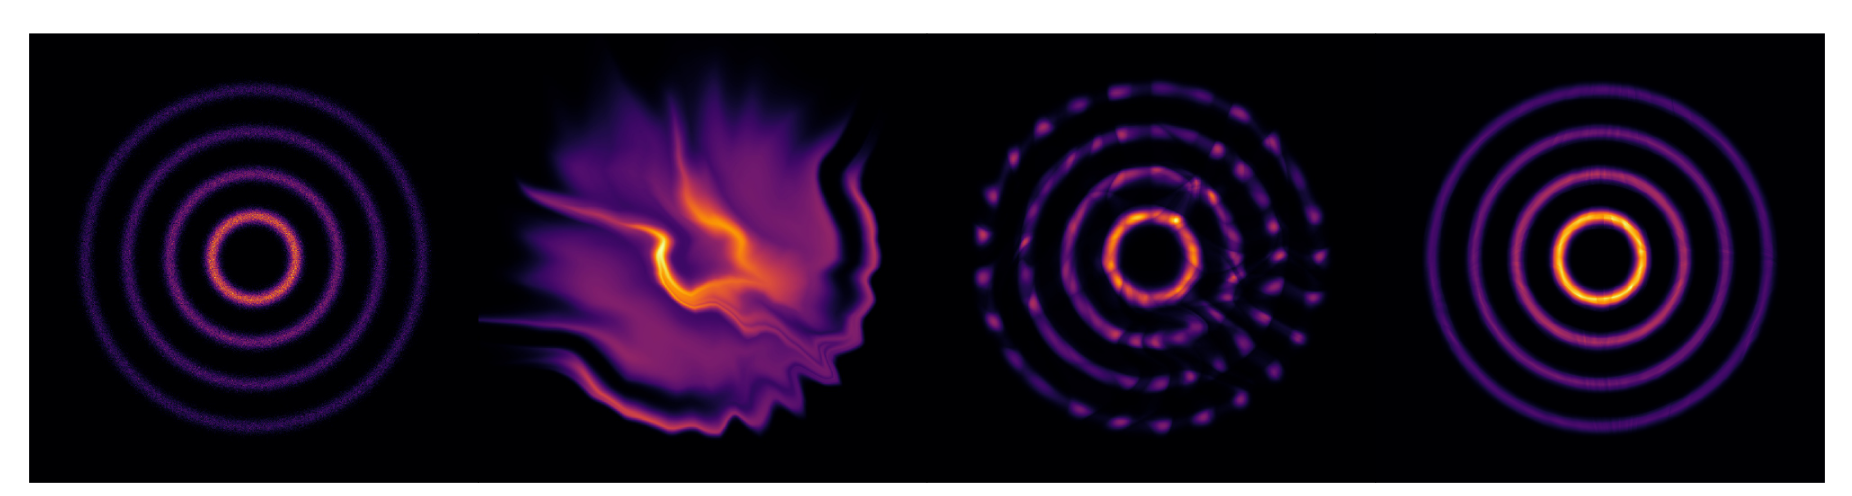
\includegraphics[width=\textwidth]{images/coupling-flow.png}
	\caption{Different normalizing flow models on a synthetic conditionally distributed dataset. From left to right: ground truth, Glow, i-ResNet, Linear Rational Splines (used in this method). Taken from \cite{dolatabadi_invertible_2020}}
	\label{fig:coupling-flow}
\end{figure}

Most importantly, these coupling flows are able to capture full joint distributions and have been used in models such as VAEs and generative models \cite{kobyzev_normalizing_2021} as seen in figure \ref{fig:coupling-flow}. Crucially, this gives an extremely flexible family of distributions that ought to be able to capture the conditional structure that exists within a graph.

More specifically, when sampling a random graph, one can begin the construction by taking a base edge and sampling a value from it. Then, to sample another edge, the distribution must be conditional on the distribution of the first edge. This process continues with each successive edge that is sampled being contingent on all preceding edges which is exactly what happens in the autoregressive transform. Hence, this is a good fit for the graph sampling problem.

\subsubsection{General Normalizing Flow Model}
In general, the normalizing flow will will operate as follows:
\begin{enumerate}
	\item A value will be sampled from a base distribution $b \sim \mathcal{B}$ with $\mathcal{B}$ being a fixed base distribution. In this case, we chose 
	\[
		\mathcal{B} = Beta(0.95, 0.95)
	\]
	in order to bias the explanation towards sparse explanations that are favored in the literature \cite{yuan_explainability_2021}.
	\item The value then gets put through a series of $m$ linear rational spline coupling normalizing flows giving the edge mask distribution. Let all the layers be denoted by $\mathcal{L}_{\mathcal{B}, \Theta}$ where $\Theta$ represents the parameters of the LRS layers. Therefore, we have
	\begin{align*}
		W_i = \sigma(\mathcal{L}_{\mathcal{B}, \Theta}(b))
	\end{align*}
	where $\sigma$ is the standard sigmoid function.
	\item Finally, we get the conditional GNN classifier $\hat{y}$ as the distribution given by
	\begin{align*}
		\hat{y} = \phi(v_i, \mathcal{X}, \mathcal{N}_l(v_i, E), W_i)
	\end{align*}
	from which we apply a learning algorithm to obtain the weights $\Theta$
	\item Once this is done, the final edge interpretation is given by
	\begin{align*}
		\mathcal{W}_i = \mathbb{E}[\sigma(\mathcal{L}_{\mathcal{B}, \Theta})]
	\end{align*}
	which is obtained simply by averaging Monte-Carlo sampling of the LRS layers.
\end{enumerate}
For the graph edge interpretation model, this is the most general Bayesian algorithm that can be given due to the universality of the LRS coupling normalizing flow. Since the graph interpretation is expected to be quite a complicated distribution, the goal of this method is to capture all of the higher order complexities, including multi-hop relationships. The listing \ref{alg:nf-model} succinctly captures this algorithm.
\begin{algorithm}[h]
	\centering
	\caption{The model setup for the Normalizing Flow model}
	\label{alg:nf-model}
	\begin{algorithmic}
		\Require $v_i \in V, \bar{\alpha} > 0, \bar{\beta} > 0$
		\Require $c \sim \phi(v_i, \mathcal{X}, \mathcal{N}_l(v_i, E), \mathcal{W})$
		\State $\mathcal{B} \gets Beta(\bar{\alpha}, \bar{\beta})$
		\State $b \sim \mathcal{B}$
		\State $W_i \gets \sigma(\mathcal{L}_{\mathcal{B}, \Theta}(b))$
		\State $\hat{y} \gets \phi(v_i, \mathcal{X}, \mathcal{N}_l(v_i, E), W_i)$
		\State $\hat{c} \sim \hat{y}$
	\end{algorithmic}
\end{algorithm}

\subsubsection{KL-Divergence and Direct Optimization}
The method used to train the parameters $\Theta$ is taking the distribution $\hat{c}$ and $c$ and backpropogating against the KL-divergence of these two distributions. Because of the reparametrization trick and the fact that the GNN is fully differentiable, this gives the gradient of the KL-divergence against $\Theta$ and allows for direct optimization against these parameters. Any SGD algorithm can be used, and, in particular, the ADAM optimizer \cite{kingma_adam_2017} is used in this model. Additionally, an L1 regularization is applied to the edge mask to enforce sparsity on the model. This ensures that the model does not converge on the full graph as its output and is forced to learn the truly important edges. 

\newpage
